\subsection{ORB-SLAM3}

ORB-SLAM3 is a KV-SLAM implementation which is popular in research contexts due to its performance, open source codebase, and usage of methods and techniques that are well-documented and widely understood.

It is difficult to conceptualize modern SLAM as a pipeline from inputs to outputs. While implementations differ significantly, KV-SLAM can be better understood as a collection of tightly coupled concurrent processes. Figure \ref{fig:subprocesses} shows a block diagram of the layers and subprocesses of a modern KV-SLAM system. A complete understanding of each subprocess is not necessary, so we offer a high level overview here, with additional detail given to processes which can be improved through the implementation of the viewpoint-aware point removal method.

\begin{figure}[!ht]
    \centering
    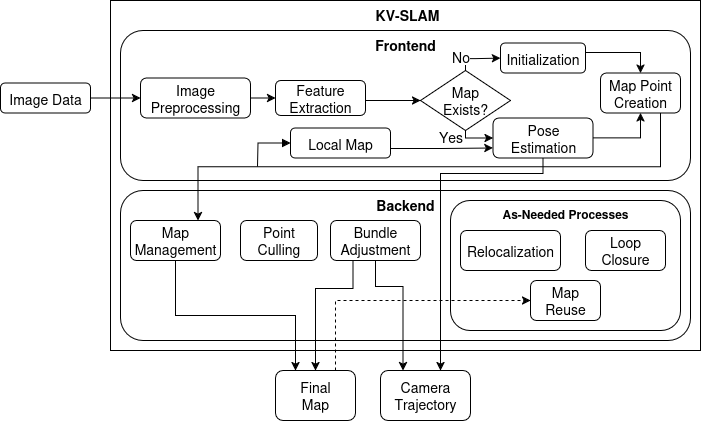
\includegraphics[width=0.9\textwidth]{resources/subprocesses.png}
    \caption[KV-SLAM Subprocesses]{The inputs, outputs, and subprocesses of a model simplified KV-SLAM system.}
    \label{fig:subprocesses}
\end{figure}

The frontend is responsible for coarse motion estimates and map point generation. It is capable of determining 3D relative motion between two images in the case of initialization, or localization within a small local map in the case of pose estimation. The frontend needs to be extremely fast, as running slower than the frame rate of the camera would lead to a backlog of images to process, and would prevent real-time performance. To that end, the frontend assumes small-scale, continuous motion between frames, and does not handle discontinuities well.

The backend is responsible for integrating the coarse motion estimates and map points from the frontend into the larger context of the global map and trajectory. There will always be some error in the motion and map point estimations from the frontend, so the backend adjusts various elements of the global estimate such as frame positions, map point positions, and camera parameters to minimize the overall error within the global estimation in an optimization process called bundle adjustment \cite{triggsBundleAdjustmentModern2000a}. The backend processes tend to run at a slower rate than the frontend, focusing on providing global consistency that the frontend cannot produce alone.

Within this model, the VD-MPR system being researched would reside in the backend, specifically under the point culling subprocess. The purpose of point culling is to reduce the overall size of the map by removing map points which are redundant, outliers, or otherwise unhelpful. There are two categories of processes which benefit from reducing the map to a minimal set of most useful, most correct data. The first is optimization processes such as bundle adjustment and PnP, where additional data and outlier data can cause the system to fail to find a consistent solution. The second category is processes which search the map, such as relocalization and loop closure.
